%
%  THESISBOEK
%
%  Dit bestand zorgt voor algemene (layout)definities, en groepeert de
%  afzonderlijke LaTeX-files tot een geheel.
%
%  @author Erwin Six, David De Reu, Brecht Vermeulen
%

\documentclass[11pt,a4paper,oneside,notitlepage]{book}
\usepackage[english,dutch]{babel}

% marges aanpassen
% (opmerking: moet *voor* inclusie van fancyhdr package komen)
\setlength{\hoffset}{-1in}
\setlength{\voffset}{-1in}
\setlength{\topmargin}{2cm}
\setlength{\headheight}{0.5cm}
\setlength{\headsep}{1cm}
\setlength{\oddsidemargin}{3.5cm}
\setlength{\evensidemargin}{3.5cm}
\setlength{\textwidth}{16cm}
\setlength{\textheight}{23.3cm}
\setlength{\footskip}{1.5cm}

\usepackage{fancyhdr}
\usepackage{graphicx}
\graphicspath{{figuren/}} % De plaats waar latex zijn figuren gaat halen.
% \usepackage[colorlinks]{hyperref}
\usepackage{url}
\usepackage{amsmath}

\usepackage{listings} 
\usepackage{color}
\definecolor{lightgray}{rgb}{.9,.9,.9}
\definecolor{darkgray}{rgb}{.4,.4,.4}
\definecolor{purple}{rgb}{0.65, 0.12, 0.82}
\lstdefinelanguage{JavaScript}{
  keywords={break, case, catch, continue, debugger, default, delete, do, else, finally, for, function, if, in, instanceof, new, return, switch, this, throw, try, typeof, var, void, while, with},
  morecomment=[l]{//},
  morecomment=[s]{/*}{*/},
  morestring=[b]',
  morestring=[b]",
  ndkeywords={class, export, boolean, throw, implements, import, this},
  keywordstyle=\color{blue}\bfseries,
  ndkeywordstyle=\color{darkgray}\bfseries,
  identifierstyle=\color{black},
  commentstyle=\color{purple}\ttfamily,
  %stringstyle=\color{red}\ttfamily,
  sensitive=true
}

\lstset{
   language=JavaScript,
   extendedchars=true,
   basicstyle=\footnotesize\ttfamily,
   showstringspaces=false,
   showspaces=false,
   %numbers=left,
   numberstyle=\footnotesize,
   numbersep=9pt,
   tabsize=2,
   breaklines=true,
   showtabs=false,
   captionpos=b,
   belowcaptionskip=1\baselineskip,
   frame=L,
   xleftmargin=\parindent,
   language=[x86masm]Assembler,
   basicstyle=\footnotesize\ttfamily,
   commentstyle=\itshape\color{black}
}

\pagestyle{fancy}

\renewcommand{\chaptermark}[1]{\markright{\MakeUppercase{#1}}}
\renewcommand{\sectionmark}[1]{\markright{\thesection~#1}}

\newcommand{\headerfmt}[1]{\textsl{\textsf{#1}}}
\newcommand{\headerfmtpage}[1]{\textsf{#1}}

\fancyhf{}
\fancyhead[LE,RO]{\headerfmtpage{\thepage}}
\fancyhead[LO]{\headerfmt{\rightmark}}
\fancyhead[RE]{\headerfmt{\leftmark}}
\renewcommand{\headrulewidth}{0.5pt}
\renewcommand{\footrulewidth}{0pt}

\fancypagestyle{plain}{ % eerste bladzijde van een hoofdstuk
  \fancyhf{}
  \fancyhead[LE,RO]{\headerfmtpage{\thepage}}
  \fancyhead[LO]{\headerfmt{\rightmark}}
  \fancyhead[RE]{\headerfmt{\leftmark}}
  \renewcommand{\headrulewidth}{0.5pt}
  \renewcommand{\footrulewidth}{0pt}
}

% anderhalve interlinie (opm: titelblad gaat uit van 1.5)
\renewcommand{\baselinestretch}{1.5}

% indien LaTeX niet goed splitst, neem je woord hierin op, of evt om splitsen 
% te voorkomen
\hyphenation{ditmagnooitgesplitstworden dit-woord-splitst-hier}

\begin{document}

% titelblad (voor kaft)
\include{titel}

% lege pagina (!!)

% titelblad (!!)

% geen paginanummering tot we aan de inhoudsopgave komen
\pagestyle{empty}

% voorwoord met dankwoord en toelating tot bruikleen (ondertekend)
\include{voorwoord}

% overzicht
%  Overzichtsbladzijde met samenvatting

\newpage

{
\setlength{\baselineskip}{14pt}
\setlength{\parindent}{0pt}
\setlength{\parskip}{8pt}

\begin{center}

\noindent \textbf{\huge
Optimalisatie van client-side\\[8pt]
intermodale routeplanning
}

door 

Brecht Van de Vyvere

Scriptie ingediend tot het behalen van de academische graad van\\
Master of Science in de industri\"ele wetenschappen: informatica

Promotor: Prof.~Erik~Mannens, Prof.~Rik~Van de Walle\\
Scriptiebegeleider: Dr.~Ir.~Ruben~Verborgh, Ing.~Pieter~Colpaert

Vakgroep Elektronica en Informatiesystemen, Vakgroep Industri\"ele Technologie en Constructie\\
Voorzitter: Prof.~Dr.~Ir.~Rik~Van de Walle\\
Faculteit Ingenieurswetenschappen en Architectuur\\
Academiejaar 2015--2016


\end{center}

\section*{Samenvatting}

% TODO: samenvatting

Routeplanning is niet meer weg te denken uit ons dagelijks leven. Is het nu voor de trein naar het werk te nemen of het vliegtuig naar je vakantiebestemming, de mogelijkheden zijn onbeperkt. In deze thesis wordt onderzocht hoe routeplanning uitbreidbaar, maar ook snel gemaakt kan worden. Sinds enkele jaren wordt transportdata gepubliceerd volgens General Transit Feed Specification (GTFS). Dankzij deze uniforme structuur kunnen er algoritmes bedacht worden om data te combineren en intermodaliteit toe te laten. Bestaande oplossingen maken gebruik van een webservice architectuur, maar dit maakt het moeilijk om te voldoen aan de eisen van de gebruiker. Linked Connections is een manier om routeplanning mogelijk te maken door het publiceren van data. Doordat de server enkel verantwoordelijk is voor het publiceren van deze connecties is deze makkelijk uitbreidbaar via hypermedia. De client zijn zelf intelligent om te beslissen welke data nodig is om een om een bepaalde route te berekenen volgens de eisen van de gebruiker. De huidige implementatie laat enkel filtering in de tijd toe waardoor de client enorm veel data moet verwerken. In deze thesis wordt een optimalisatie ge�ntroduceerd door het toepassen van geolocatie filtering.

\section*{Trefwoorden}

% TODO: trefwoorden

Linked Connections, routeplanning, optimalisatie, GTFS

}

\newpage % strikt noodzakelijk om een header op deze blz. te vermijden


\pagestyle{fancy}
\frontmatter

% inhoudstafel
\tableofcontents

% opmaak voor het eigenlijke boek; onderstaande lijnen
% weglaten als de eerste regel van een nieuwe alinea moet
% inspringen in plaats van extra tussenruimte
%\setlength{\parindent}{0pt}
%\setlength{\parskip}{0.5\baselineskip plus 0.5ex minus 0.2ex}
%\setlength{\parskip}{1ex plus 0.5ex minus 0.2ex}

% hoofdstukken
\mainmatter

% hier worden de hoofdstukken ingevoegd (\includes)

\chapter{Inleiding}

\section{Probleemstelling}

\subsection{Routeplanning}
Huidige routeplanners worden klassiek ge\"implementeerd met een Application Programming Interface (API). Dit houdt in dat de server bepaalde functionaliteiten aanbiedt aan de client zonder dat de client weet hoe die werkelijk werkt. Voor veel vervoersmaatschappijen is routeplanning niet meer dan een gegevensbank opzetten en een applicatie hiermee bouwen. Listing \ref{klassieke-webservice-interface} toont hoe een typische XML/JSON API eruit ziet waarbij je een aantal parameters moet invullen om een route te laten berekenen.\\

\begin{lstlisting}[label=klassieke-webservice-interface,caption=Klassieke webservice interface]
http://my-api.org?start={...}&bestemming={...}&transportmodes={...}&extraFeature={...}&...
\end{lstlisting}

Dankzij de hulp van organisaties die open data stimuleren wordt transportdata, maar ook andere data opengesteld. Dit biedt tal van mogelijkheden om meer gepersonaliseerde routeplanners te ontwerpen, bijvoorbeeld een routeplanner die rekening houdt met rolstoeltoegankelijkheid. Om deze functionaliteit toe te voegen aan de klassieke routeplanner API moeten er extra parameters meegegeven worden. Deze manier van werken is moeilijk uitbreidbaar doordat intelligentie gecentraliseerd zit in de server en er een sterke koppeling tussen cli\"ent en server bestaat.

%\vspace{3mm} %5mm vertical space

Met gelinkte connecties (Engels: \textit{Linked Connections}) is het mogelijk voor cli\"ents om zelf functionaliteit te ontdekken. Hierbij is de cli\"ent en server losgekoppeld. Het is de verantwoordelijkheid van de cli\"ent om een route te berekenen via de data die ter beschikking gesteld wordt door de server. Dit gaat ten koste van bandbreedte en snelheid. Momenteel is het zo dat hoe langer de afstand is en/of meerdere transportmodi, hoe langer het duurt voor een route te berekenen (zie resultaten 5.1). Om Linked Connections als een volwaardige oplossing te kunnen gebruiken, moet er een oplossing bedacht worden om sneller het gewenste resultaat te bekomen.

\section{Doelstelling}

Deze thesis heeft als doelstelling om client-side routeplanning met gelinkte connecties binnen redelijke tijd te kunnen berekenen. Vooral routes met lange afstanden en verschillende modi zijn een bottleneck voor de huidige implementatie. 
Als deze optimalisatie positief uitvalt zou dit werkelijk een belangrijke stap kunnen betekenen voor het Web en de Open Data wereld.


\chapter{Literatuurstudie}

\section{Dienstregeling openbaar vervoer}

Interoperabiliteit van datasets is belangrijk voor routeplanning. Zo kan een dataset van de Belgische spoorwegmaatschappij niet alleen een oplossing bieden voor Belgi\"e, maar ook voor de buurlanden. 

\subsection{GTFS}
In 2011 introduceerde Google de General Transit Feed Specification (GTFS) \cite{gtfs-ref}. Dit is een set van regels die vervoermaatschappijen moeten volgen om hun tijdstabellen te publiceren. Simpelweg beschrijft het welke CSV-bestanden ge�ncludeerd moeten worden en welke headers verplicht en optioneel zijn per bestand. 
Vervoersmaatschappijen zoals De Lijn, NMBS, NS \footnote{Nederlandse Spoorwegen} etc. hebben dit al opgesteld.

\begin{itemize}
	\item trips.txt Een trip is een traject die een voertuig aflegt van de eerste stopplaats tot en met de laatste stopplaats. Dit bestand zorgt voor de mapping tussen trip, een route en service.
	\item routes.txt Een route is een verzameling trips. Een trip volgt een bepaalde route, maar kunnen verschillende stopplaatsen hebben. Door met routes te werken kan er makkelijk meer informatie toegevoegd worden over al deze trips zoals rolstoeltoegankelijkheid.
  	\item calendar.txt Dit bestand bevat net als een kalender welke dagen van maandag tot en met zondag een bepaalde service rijdt. Een service is niet meer dan een verzameling datums een bepaalde  route rijdt.
   	\item calendar\_dates.txt Dit bevat uitzonderingsdagen dat een service niet of juist wel rijdt, bijvoorbeeld wegens een feestdag. Wegens de complexiteit van een calendar.txt op te stellen, gebruiken vervoermaatschappijen meestal enkel een calendar\_dates.txt bestand met daarin alle dagen dat services actief zijn als uitzondering toegevoegd.
    	\item stoptimes.txt Deze bestaat uit een verzameling stopplaatsen met telkens de aankomst- en vertrektijden bij.
	\item stops.txt Bevat een lijst met informatie over alle stopplaatsen. Deze wordt gebruikt om twee datasets te koppelen met elkaar op basis van de afstand tussen stops.
\end{itemize}

Verder bevat GTFS regels over de prijsregeling van tickets of de co\"ordinaten van het traject van een trip zelf, maar deze zijn nog niet van toepassing voor gelinke connecties.

\subsection{GTFS-RT}

GTFS-RealTime is een extra laag bovenop GTFS data. Deze bevat informatie over vertragingen, omleidingen etc. Deze is momenteel niet ge\"implementeerd in gelinkte connecties zou een latere uitbreiding kunnen vormen (zie future work).

\section{Semantisch web}

Het semantisch web is een verzameling technologi\"een (URI, RDF, SPARQL, ontologi\"en...) die het mogelijk maakt om informatie op het web machine-leesbaar te maken. Concepten, termen en relaties binnen een bepaald domein worden met elkaar gelinkt waardoor het mogelijk is om meer informatie te weten te komen dan aanvankelijk aanwezig aanwezig was.

\subsection{RDF}

Resource Description Framework (RDF) is een conceptueel model om bronnen op het web weer te geven. Feiten worden opgebouwd met een drieledige structuur: subject - predikaat - object. Dit geeft meer flexibiliteit dan bijvoorbeeld een relationeel model in object geori�nteerd programmeren. Een van de grote voordelen is dat je uit deze feiten nieuwe feiten kunt halen. 

Bv. : Trein 123 heeft als aanduiding `Brussel - Gent'.\\
$\rightarrow$ Subject:  Trein 123 - Predikaat: aanduiding - Object : `Parijs'

\includegraphics[scale=0.5]{ruglogo.pdf}

Een RDF model is dus een gerichte graaf waarbij de knopen en verbindingen benoemd zijn. Er ontstaat als het ware een web van verschillende concepten die met elkaar verweven worden. 

\subsection{Vocabulariums}
Een vocabularium is een verzameling klasses, eigenschappen die met elkaar verbonden worden binnen een bepaalde context. RDF is een vocabularium op zich waarbij bronnen ofwel een subject, predikaat of object voorstellen. Er wordt geen rekening gehouden met de context. We willen net zoals bij OOP klasses maken die bepaalde functionaliteit voorstellen. RDFS (Resource Description Framework Schema) en OWL (Web Ontology Language) bieden hier een oplossing voor. Met RDFS worden er extra elementen ge�ntroduceerd waarmee er gespecificeerd kan worden of een bron een klasse, eigenschap, waarde of datatype voorstelt.

Bij ons voorbeeld kunnen we een nieuwe klasse Trein introduceren, waartoe Trein 123 behoort. Met de type-property van de RDF vocabularium kunnen we het type specificeren:
?Trein 123? rdf:type Trein
Zo kunnen we ook voor het predikaat ?aanduiding? aangeven dat deze als subject een instantie van het type Klasse verwacht en als object een instantie van een klasse Station.

\subsection{Bronidentificatie}
Met RDF hebben we een model om bronnen met elkaar te linken en zo feiten te cre�eren. Met HTTP URI?s (Universal Resource Identifiers) worden bronnen eenduidig ge�dentificeerd zodat er geen verwarring kan ontstaan. Bijv.: https://example.org/books/123
Dit heeft als voordeel dat sommige URI?s in feite een URL (Universal Resource Locators) zijn. Dit wil zeggen dat je kunt surfen naar die link en zo meer informatie te weten kan komen, net alsof je een website zou bezoeken in je browser.

Om niet telkens de volledige URI te moeten typen wordt er gebruik gemaakt van prefixen. Volgende prefix wordt gebruikt in de voorbeelden:
PREFIX vb: <http://voorbeeld\#>

\subsection{Re\"ificatie}

Nu dat we een collectie triples hebben, willen we meer informatie over bepaalde triples zelf. (Is het mogelijk om alle triples met bepaald subject of subject+predikaat te re\"ificeren?) Om dit te kunnen doen wordt de triple in zijn geheel als bron behandeld. Dit proces wordt re�ficatie genoemd.
Stel, we hebben volgende triple: subject: ?ex:trein123?, predikaat: ?ex:isGestationeerdIn?, object: ?ex:Rijsel?. Voor een transportbedrijf kan het handig zijn om te weten welke conducteur de trein heeft gestationeerd. Om deze informatie toe te voegen aan de triple, wordt er een subject gemaakt met als type rdf:statement:

\begin{lstlisting}[label=reificatie,caption=Re\"ificatie van een triple]
ex:treinStationering1            rdf:type    rdf:statement
ex:treinStationering1            rdf:subject    ex:trein123
ex:treinStationering1            rdf:predicate    ex:isGestationeerdIn
ex:treinStationering1            rdf:object    stations:Rijsel
ex:treinStationering1        rdf:conducteur    conducteurs:1
\end{lstlisting}

Nu hebben we een attribuut toegevoegd over onze oorspronkelijke triple. Wat we willen is een context toevoegen aan een collectie triples. Een context wordt net als een andere bron ge�dentificeerd met een URI. Deze wordt simpelweg als attribuut toegevoegd aan de triples.

Dit zorgt uiteraard voor onnodig veel extra triples:

TO = aantal originele triples
TN = aantal nieuwe triples
$\rightarrow$ TN = 3 x TO + 1

\subsection{Linked Data}

\subsection{Linked Data Fragments}



\section{REST}

\subsection{Principes}

\subsection{Hypermedia}



\section{Bestaande routeplanners}

\subsection{Dijkstra}

\subsection{Transitland}

\subsection{Navitia}

\chapter{Linked Connections}
\label{lc}

Linked Connections \cite{colpaert_iswc_2015} is een framework die \textit{client-side} routeplanning mogelijk maakt. Volgende sectie verduidelijkt hoe de huidige implementatie werkt. Vervolgens wordt uitgelegd hoe connecties worden gegenereerd uit een GTFS feed. Ten slotte wordt verduidelijkt hoe intermodaal routeplannen werkt.

\section{Principe}

Stel je voor dat je de tram moet nemen naar je werk: je stapt ergens op, wacht vijf stophaltes en aan de zesde stophalte stap je af. Dit is een route die uit zes connecties bestaat. Een connectie is de verbinding tussen een vertrek- en eindstop zonder onderbreking. Bij zo'n connectie horen respectievelijk ook een vertrek- en aankomsttijd. Een route kan berekend worden met het CSA algoritme (zie \ref{csa}) die een query en een gesorteerde lijst op vertrektijd als inputwaarde vereist.

Een Linked Connections server presenteert deze gesorteerde connecties in de vorm van Linked Data Fragments (\ref{ldf}) aan de cli\"ent. Momenteel is het enkel mogelijk om de vertrektijd van een query mee te geven als parameter. Met behulp van texttit{hydra:nextPage} links kan de cli\"ent makkelijk opeenvolgende fragmenten ophalen. (zie figuur \ref{lcfragmenten}).

\begin{figure}[h!]
\centering
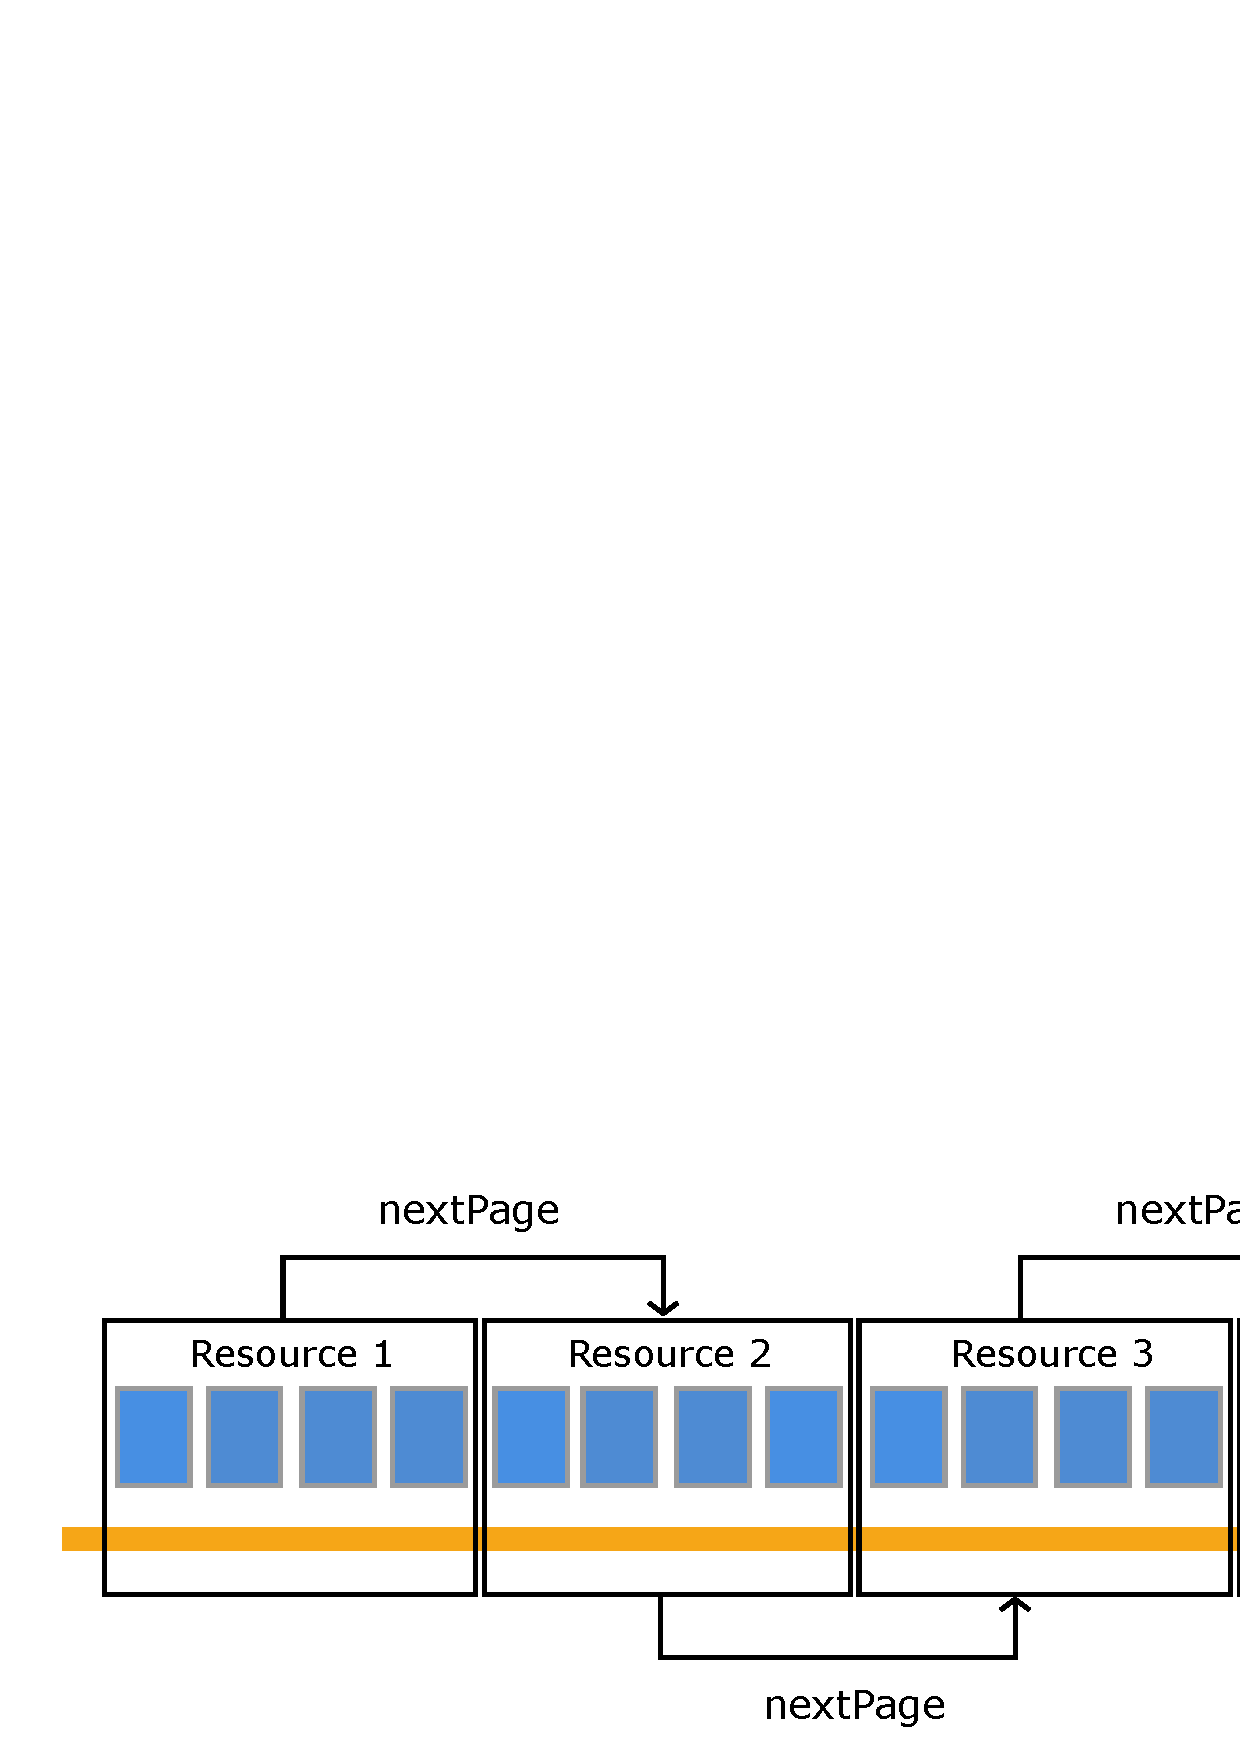
\includegraphics[width=0.8\textwidth]{hypermediafragmenten.png}
\caption{Connecties zijn gesorteerd onderverdeeld in fragmenten die verbonden zijn met hydra:nextPage links.}
\label{lcfragm}
\end{figure}

\begin{lstlisting}[label=queryconnecties,caption=HTTP URL van fragment met Linked Connections.]
http://voorbeeld.org/connecties?vertrekTijd=2015-10-21T11\%3A30
\end{lstlisting}

Het publiceren van de data gebeurt met behulp van drie technologi\"een: 
\begin{itemize}
\item REST zorgt ervoor dat resources cachebaar zijn. Hier zijn fragmenten de resources. Het aantal mogelijke URI's is afhankelijk van het tijdsinterval van de fragmenten. Als T het tijdsinterval in minuten is van de fragmenten, dan kan het aantal mogelijke URI's berekend worden met formule \ref{lc:aantalurisoorspronkelijk}.
\begin{equation} \label{lc:aantalurisoorspronkelijk}
24 * 60 / T
\end{equation}

Als T = 10 min, dan zijn er 144 verschillende fragmenten. De meeste ov-bedrijven rijden niet 24/24 dus in praktijk zijn er nog minder fragmenten. Met behulp van HTTP omleidingen kan dit opgelost worden.
\item Hypermedia zorgt niet enkel voor het vinden van volgende fragmenten, maar ook voor het makkelijk uitbreiden van connecties. Dit kan gaan van een koppeling met geonames tot koffiebars in de buurt.
\item Het semantisch web zorgt voor de semantische interoperabiliteit van de connecties en de API. Dit laat toe om generische clients te bouwen.
\end{itemize}

Op de LDF-as (zie \ref{ldf-lc5}) staat huidige implementatie aan de linkerkant. Het kost de server weinig moeite om data te publiceren door de hoge cachebaarheid. Een cli\"ent moet daarentegen veel connecties scannen om tot een route te komen. Later (\ref{resultaat-origineel}) zal de exacte performantie verduidelijkt worden.

\begin{figure}[h!]
\centering
\includegraphics[width=0.8\textwidth]{LDF-as5.png}
\caption{Linked Data Fragmenten-as met Linked Connections}
\label{ldf-lc5}
\end{figure}

\section{Voorbewerking}

Gelinkte connecties worden berekend uit een GTFS \textit{feed}. De convertor in deze masterproef maakt gebruik van een MySQL-databank om queries op uit te voeren. \footnote{Ondertussen is een veel snellere convertor gemaakt die volgens een ander principe werkt, zonder databank. Zie github.com/linkedconnections/gtfs2lc} Het is belangrijk op te merken dat connecties niet gesorteerd moeten zijn bij het voorbewerken. Deze worden later in de databank van de Linked Connections server ingeladen die zelf sorteert. Figuur \ref{inladengtfs} toont een overzicht van de verschillende stappen om connecties te genereren.

\begin{figure}[h!]
\centering
\includegraphics[width=1.0\textwidth]{Preprocessor.png}
\caption{Overzicht hoe connecties worden gegenereerd uit een GTFS feed. Deze wordt ingeladen in een MySQL databank. Met de scripttaal PHP worden connecties gegenereerd hieruit.}
\label{inladengtfs}
\end{figure}

Connecties worden dag per dag berekend. Ofwel worden start- en einddatum meegegeven als parameters, ofwel worden start- en einddatum van de GTFS feed zelf genomen. Vervolgens worden alle services uit \textit{calendar} en \textit{calendar\_dates} van een bepaalde dag opgehaald. Bij elke service hoort een bepaalde \textit{route} en een verzameling \textit{trips} die dan worden opgehaald uit \textit{trips}.
Een laatste stap is het overlopen van \textit{stoptimes.txt}. Uit de combinatie van twee opeenvolgende stoptimes kan een connectie berekend worden. Lijst \ref{vbstoptimes} bevat een voorbeeld van twee opeenvolgende stoptijden van een bepaalde trip.

\begin{lstlisting}[label=vbstoptimes,caption=Vereenvoudigde stoptimes in CSV.]
trip_id,arrival_time,departure_time,stop_id,stop_sequence
16,07:18:00,07:18:00,8200100,1
16,07:33:00,07:33:00,8200110,2
\end{lstlisting}

\begin{figure}[h!]
\centering
\includegraphics[width=0.8\textwidth]{volgordeconvertor.png}
\caption{Per dag worden de corresponderende service ID's, trip ID's en route ID's berekend. De vertrek-/aankomststopplaats met respectievelijk vertrek-/aankomsttijd worden berekend uit een verzameling stoptimes. }
\end{figure}

Codevoorbeeld \ref{connectiejsonld} toont hoe een connectie eruit ziet bij output. Merk op dat een '@context' niet is toegevoegd en ook niet in een graaf zit. In subsectie \ref{jsonldstream} wordt hierover meer uitleg gegeven.

\begin{lstlisting}[label=connectiejsonld,caption=Connectie voor een bepaalde trip met bijkomstige route in JSON-LD.]
{	
	"@id": "http://example.org/connections/1"
	"@type": "http://semweb.mmlab.be/ns/linkedconnections#Connection",
	"http://vocab.gtfs.org/terms#trip": "16",
	"http://vocab.gtfs.org/terms#route": "route-1",
	"http://semweb.mmlab.be/ns/linkedconnections#departureTime": "2015-10-21T06:18:00.000Z",
	"http://semweb.mmlab.be/ns/linkedconnections#departureStop": "8200100",
	"http://semweb.mmlab.be/ns/linkedconnections#arrivalTime": "2015-10-21T06:33:00.000Z",
	"http://semweb.mmlab.be/ns/linkedconnections#arrivalStop": "8200110"
}
\end{lstlisting}

De tijdszone van vertrek- een aankomsttijd staat in Coordinated Universal Time (UTC). Er moet altijd rekening gehouden worden met de tijdszone van de GTFS feed. In dit voorbeeld \ref{vbstoptimes} werd een feed uit Belgi\"e genomen. Om de Belgische tijd (UTC+1) om te zetten naar UTC moet er een uur afgetrokken worden van de tijd die vermeld staat in GTFS stoptijden.

Een van de moeilijkheden voor het genereren van connecties was het ophalen van trips die voor middernacht vertrekken, en dus geclassificeerd zijn onder die dag, maar na middernacht pas stoppen. GTFS lost dit op door de tijd na middernacht door te tellen, bijvoorbeeld 2u 's nachts staat weergegeven als 26u. Volgens GTFS rijden deze stoptimes allemaal op dezelfde dag, maar voor Linked Connections zijn dit effectief twee verschillende dagen, omdat er met exacte tijden gewerkt wordt.
Om dit op te lossen worden er twee extra vlaggen toegevoegd in de databank of de vertrek- en aankomsttijd van een stoptijd voor of na middernacht plaatsvinden.

Een databank gebruiken heeft als grote nadeel dat de data ingeladen moet worden vooraleer berekeningen kunnen plaatsvinden. In \ref{table:inladengtfs} staat een overzicht van de drie gebruikte datasets in deze masterproef met de tijd om in te laden. Voor zeer grote datasets, zoals De Lijn, is inladen een bottleneck.

\begin{table}[htbp]
\centering
\begin{tabular}{ | l || c | c | c |}
  \hline			
    & Tijd (min) & Grootte (MB) & Periode (weken) \\ \hline
  NMBS & 3.1 & 1.1 & 12  \\
  NS & 8.35 & 21.4 & 56 \\
  De Lijn & 100 & 44 & 10 \\
  \hline  
\end{tabular}
\caption{Tijd om een GTFS feed in te laden in een MySQL databank.}
\label{table:inladengtfs}
\end{table}

Het genereren van connecties zelf gaat een stuk rapper. In \ref{table:connectiesgenereren} zie je dat voor kleine datasets (zoals NMBS en NS) het minder dan minuut duurt om de connecties voor een dag te berekenen. De Lijn scoort opnieuw zeer slecht door de grootte van de dataset.

\begin{table}[htbp]
\centering
\begin{tabular}{ | l || c | c | c |}
  \hline			
    & Tijd (min) & Connecties \\ \hline
  NMBS & 0.21 & 55479 \\
  NS &  &  \\
  De Lijn & 14.97 & 1049186 \\
  \hline  
\end{tabular}
\caption{Tijd om connecties te genereren voor een dag.}
\label{table:connectiesgenereren}
\end{table}

\subsection {JSON-LD stream}
\label{jsonldstream}
Om de connecties als Linked Data te publiceren werd er voor gekozen om JSON-LD te gebruiken. JSON wordt beschouwt als het \textit{de facto} standaardformaat op het web dankzij de compactheid, leesbaarheid en vele handige tools die hiervan gebruik maken. Wanneer een verzameling objecten dezelfde context heeft, zijn er twee mogelijkheden om deze te publiceren:
\begin{itemize}
\item een gemeenschappelijke context voorzien en alle objecten in bijhorende graaf steken (zie \ref{tripjsonldgraph}). Deze methode vereist dat de graaf in het geheugen geladen moet worden vooraleer verdere operaties mogelijk zijn.
\item elk object een context geven (zie \ref{tripjsonld}). Met deze methode kan object per object gestreamt worden, maar zorgt voor grote overhead door de context die telkens mee gepubliceerd wordt.
\end{itemize}
Een oplossing hiervoor is de JSON-LD streamspecificatie \footnote{https://github.com/pietercolpaert/jsonld-stream}. Deze geeft aan dat de context van een object met '@context' van toepassing is op alle andere objecten van het document. Zo moet er maar eenmalig een context opgegeven worden en wordt impliciet verondersteld dat de andere objecten deze context gebruiken.
De voorbewerker kan nu connecties als Linked Data wegschrijven zonder extra dataverlies en gestroomlijnd. Dit stroomlijnen is belangrijk om de data later lijn per lijn te kunnen inladen in een databank.

\section{Client}

De client is verantwoordelijk voor het berekenen van de snelste route. Deze kan met een paar lijntjes code aangemaakt worden (zie \ref{clientvb}).
\begin{lstlisting}[label=clientvb,caption=Code om client op te zetten in JavaScript.]
var planner = new window.lc.Client({"entrypoints" : ["http://example.linkedconnections.org/"]});
planner.query({
			"departureStop": "Brussel-Zuid",
			"arrivalStop": "Gent-Sint-Pieters",
			"departureTime": new Date("2015-11-05T10:00")
			}, function (stream) {
				stream.on('result', function (pad) {
					// pad bevat verzameling connecties die snelste route voorstellen
				});
			 	stream.on('data', function (connectie) {
			 		// connectie is gebruikt geweest voor minimale overspannende boom
			 	});
});
\end{lstlisting}
\label{vbclient}

Linked Connections van verschillende ov-bedrijven worden gedistribueerd opgesteld. De cli\"ent is verantwoordelijk voor het samenvoegen van connecties. In figuur \ref{overzichtclientserver} staat een overzicht van een client - meerdere servers opstelling. Rechts staan twee Linked Connection servers, de ene verantwoordelijk voor de connecties van een vervoersmaatschappij van bussen, de andere van treinen. Links staat een client die de fragmenten ophaalt van beide servers. Voor het scannen zelf kan plaatsvinden, moeten deze samengevoegd worden. Daarna kan de snelste route met Connection Scan Algorithm (CSA) gepland worden.

\begin{figure}[h!]
\centering
\includegraphics[width=0.5\textwidth]{OverzichtClientServer.png}
\label{overzichtclientserver}
\caption{Opstelling van een client en twee Linked Connections servers.}
\end{figure}

\subsection{Merger}

Een merger voegt meerdere stromen van gesorteerde connecties samen tot een stroom. Dit is noodzakelijk voor de cli\"ent om CSA te kunnen toepassen.

Connecties komen onder de vorm van een \textit{stream} binnen. Zo'n stream werkt asynchroon met events. Deze worden opgeworpen wanneer bijvoorbeeld data beschikbaar is. Figuur \ref{merger} toont een overzicht van een merger. Deze luistert (1) naar de verschillende datastromen tot deze data vrijgeven. De connecties worden toegevoegd in wachtrijen. Wachtrijen (2) hebben als voorwaarde dat ze zelf gesorteerd zijn. Datastromen worden telkens gepauzeerd na het opvangen van data. Dit is noodzakelijk om de cli\"ent beslissingstijd te geven. Zo kan er beslist worden om een bepaalde connectiestroom uit te schakelen of toe te voegen. Een andere reden waarom de merger de connectiestromen pauzeert, is het feit dat de wachtrijen minstens een connectie moet bevatten van elke connectiestroom. Wanneer de merger connecties teruggeeft, worden alle connecties van elke wachtrij met dezelfde lokaal minimale vertrektijd teruggegeven. Zo blijven alle wachtrijen synchroon.

\begin{figure}[h!]
\centering
\includegraphics[width=0.5\textwidth]{merger.png}
\caption{Overzicht merger}
\label{merger}
\end{figure}

\begin{lstlisting}[label=vbclient,caption=Voorbeeldcode van een merger. Deze voegt meerdere stromen van connecties samen.]
"var connectionsStreams = [
    [ 'stream1', connectionsReadStream1 ],
    [ 'stream2', connectionsReadStream2 ],
    ...
];

var connectionsReadStream = new csa.MergeStream(connectionsStreams, query.departureTime);"
\end{lstlisting}

\section{Voor- en nadelen}

\begin{itemize}
\item Routeplanning is een dataprobleem geworden. Datapubliceerders zijn verantwoordelijk voor het publiceren van connecties en bijhorende data. Zo kan er makkelijk data toegevoegd worden via hypermedia: \textit{point of interests}, rolstoelvriendelijkheid etc. De cli\"ent bepaalt zelf welke informatie deze wil gebruiken.
\item Connecties zijn makkelijk distribueerbaar over meerdere servers. 
\end{itemize}

\chapter{Optimalisatie}
\label{opt}

\begin{figure}[h!]
\centering
\includegraphics[scale=0.4]{LDF-as4.png}
\caption{Linked Data Fragmenten-as met Linked Connections optimalisatietechniek}
\end{figure}

\section{Geofiltering}

\section{Server}

\subsection{Cachebaarheid}

Aantal mogelijke URI's voor 1 dag met enkel tijdsfilter en fragmenten om de 10 minuten:
24u * 60 min / 10 min = 144 URI's
\subsection{Grootte fragmenten}

Hoeveel connecties per fragment best?
Hangt samen met snelheid
Snelheid requests < snelheid verwerken connecties ? Is er bottleneck?

Verhouding aantal connecties/request -> tijdsinterval aanpassen

\subsection{Burenconnecties}

\section{Client}

\subsection{Heuristiek}

\begin{figure}[h!]
\centering
\includegraphics[scale=0.5]{HeuristiekClient.png}
\caption{Heuristiek client voor volgende vertrekstop}
\end{figure}


\section{Voor- en nadelen}

\chapter{Resultaten}
%\label{resultaten-origineel}

In dit hoofdstuk bespreken we de testen die een antwoord geven op de onderzoeksvraag en hypotheses. In sectie \ref{opstelling} worden enkele praktische zaken besproken. Daarna worden de drie besproken technieken uit hoofdstukken \ref{blcf} en \ref{nlcf} onderling vergeleken.

\section{Opstelling}
\label{opstelling}
Deze masterproef maakte gebruik van de offici\"ele GTFS dataset van de Belgische spoorwegenmaatschappij NMBS. 

Zowel de cli\"ent als de server werden getest op dezelfde machine: een Macbook Pro 2015 editie met 8 GB RAM en Intel Core i5 2,7 Ghz processor. De cli\"ent is een webapplicatie waarin queries werden uitgevoerd. Als browser werd Firefox gebruikt.

%\begin{itemize}
%\item NMBS: de Belgische spoorwegen
%\item NS: de Nederlandse spoorwegen
%\item De Lijn: busnetwerk in Vlaanderen
%\end{itemize}

%Eerst zullen we testen hoe basic LDF scoort bij de NMBS afzonderlijk. Daarna testen we de \textit{merger} (zie \ref{merger}) uit door NMBS en NS samen te voegen. 
%Als slot kun we onze benchmarks op de dataset van De Lijn uitvoeren. Deze laatste bestaat uit een groter netwerk van stops dan NMBS en NS samen en bevat een grotere hoeveelheid connecties per dag.

%\section{Interoperabiliteit}
%Om meerdere operatoren te kunnen gebruiken is er een mapping van stops die dicht bij elkaar liggen nodig. Een use case in de praktijk moet rekening houden met bepaalde overstaptijden (Engels: \textit{transfer time}). Wegens de complexiteit van deze stops wordt dit achterwege gelaten en wordt er een minimale overstaptijd van 0 minuten ingesteld. Stops die op een afstand van minder dan 200 meter liggen, krijgen een nieuwe stop identifier, zogenaamde connectie stop identifier. Een afstand van 200 meter is nodig, omdat bushaltes van een groot station zoals Antwerpen-Centraal ver uit elkaar liggen.
%Dit mappen naar een connectie stop identifier gebeurt voor het genereren van connecties.
%
%\section{Opstelling}
%Voor elke dataset is een Docker-container opgezet. Dit zijn virtuele machines waarin de software kan lopen. De cli\"ent is een webapplicatie die in het hoofdbesturingssysteem draait. De testen zijn uitgevoerd op een Macbook Pro 2015 editie met 8 GB RAM en Intel Core i5 2,7 Ghz.

% todo tekening docker

\subsection{Lokale server versus productieserver}

Doordat de testen werden uitgevoerd in een lokale omgeving zullen we testen of er een merkbaar verschil in snelheid is met een server in productie\footnote{Linked Connections server te vinden op: http://belgianrail.linkedconnections.org/connections/}. 
Er werden een honderdtal queries op de dataset van de NMBS uitgevoerd. Beide servers hebben als  tijdsinterval tien minuten.

\begin{table}[htbp]
\centering
\begin{tabular}{ | c || c | c | c | c | c | }
  \hline
  Type & Aantal queries & Querytijd (s) & Requests & Querytijd/request (s) & Connecties \\ \hline
  lokaal & 30 & 103.196 & 583 & 0.17 & 10368 \\
  productie & 30 & 68.5509 & 550 & 0.12 & 9915 \\
\hline  
\end{tabular}
\caption{Vergelijking tussen een lokale server een productieserver.}
\label{table:vglservers}
\end{table}

Figuur \ref{table:vglservers} toont aan dat er een verschil in snelheid is tussen een lokale en een productieserver. Dezelfde queries werden berekend met een verschillende vertrekdatum. Dit is de reden waarom het aantal requests en connecties niet gelijk zijn.
Het resultaat toont aan dat lokale server 30\% trager dan een productieserver is. Volgende subsectie toont aan welke fragmentgrootte gemiddeld het snelst is.

%\subsection{Scannen versus requests}
%
%De cli\"ent is verantwoordelijk voor het ophalen van connecties met HTTP requests die vervolgens gescant worden door CSA. Volgende hypothese wordt beantwoord:
%
%\begin{itemize}
%\item \emph{}
%\end{itemize}


\subsection{Fragmentgrootte}
\label{fragmentgrootte}

\textit{Basic Linked Connections Fragment's} (BLCF) hebben een vast tijdsinterval waarin connecties worden teruggeven. Dit komt met een gemiddeld aantal connecties. Tabel \ref{table:grootte-tijd} toont een overzicht van verschillende fragmentgroottes die mogelijk zijn met de hoeveelheid data die er gemiddeld aan verbonden is.

%\begin{table}[htbp]
%\centering
%\begin{tabular}{ | c || c | c | c | c | c | c | c | }
%  \hline
%  & \multicolumn{2}{|c|}{NMBS} & \multicolumn{2}{|c|}{NS} & \multicolumn{2}{|c|}{De Lijn} \\ \hline
%  t (min) &	Grootte (MB) &	Connecties & Grootte & Aantal connecties & Grootte & Connecties \\ \hline
% 1 &	0.012 & 56 & 0.017 & 46 & 0.25 & 975 \\
% 2 &	0.027 & 115 & 0.029 & 104 & 0.49 & 1904  \\
% 5 & 0.069 & 264 & 0.068 & 262 & 1.23 & 4833 \\
%10 &	0.14 & 570 & 0.13 & 522 & 2.47 & 9603 \\
%20 &	0.27 & 1144 & 0.25 & 1019 & 4.21 & 16441 \\
%30 & 0.41	& 1704 & 0.37 & 1539 & 6.23 & 24813 \\
%40 &	0.55	& 2281 & 0.51 & 2045 & 8.33 & 33309 \\
%80 &	1.10	& 4564 & 1.00 & 4126 & 18.71 & 66432 \\
%120 & 1.90 & 7356 & 1.51 & 6267 & 27.29 & 100314 \\
%160 & 2.21 & 9332 & 2.04 & 8075 & 35.82 & 135960 \\
%200 & 2.77 & 11419 & 2.56 & 10512 & 44.37 & 169619 \\	
%\hline  
%\end{tabular}
%\caption{Grootte (MB) en aantal connecties afhankelijk van tijdsinterval van basic LCF.}
%\label{table:grootte-tijd}
%\end{table}

\begin{table}[htbp]
\centering
\begin{tabular}{ | c || c | c | c | c | c | c | c | }
  \hline
  & \multicolumn{2}{|c|}{NMBS} \\ \hline
  t (min) &	Grootte (MB) &	Connecties \\ \hline
 1 &	0.012 & 56  \\
 2 &	0.027 & 115  \\
 5 & 0.069 & 264  \\
10 &	0.14 & 570  \\
20 &	0.27 & 1144 \\
30 & 0.41	& 1704  \\
40 &	0.55	& 2281  \\
80 &	1.10	& 4564  \\
120 & 1.90 & 7356  \\
160 & 2.21 & 9332  \\
200 & 2.77 & 11419  \\	
\hline  
\end{tabular}
\caption{Grootte (MB) en aantal connecties afhankelijk van tijdsinterval van basic LCF.}
\label{table:grootte-tijd}
\end{table}

\begin{figure}[!tbp]
  \centering
  \subfloat[De gemiddelde tijd in seconden om queries uit te voeren in functie van het tijdsinterval van basic LCF.]{\includegraphics[width=0.5\textwidth]{relatie-tijdsinterval-tijdperquery}\label{fig:relatie-tijdsinterval-tijdperquery}}
  \hfill
  \subfloat[De hoeveelheid opgevraagde data in megabyte in functie van het tijdsinterval van basic LCF.]{\includegraphics[width=0.5\textwidth]{relatie-tijdsinterval-grootte}\label{fig:relatie-tijdsinterval-grootte}}
  \caption{Snelheid en grootte hangen af van de ingestelde tijdsinterval van basic Linked Connections Fragments.}
  \label{fig:fragmentgrootte}
\end{figure}

Om te bepalen wat de optimale fragmentgrootte is, werden een honderd queries uitgevoerd met telkens een andere fragmentgrootte. De resultaten in \ref{fig:fragmentgrootte} tonen aan dat een tijdsinterval tussen 10 en 30 minuten de gemiddeld beste querysnelheid geeft. Dit komt overeen met een paginagrootte van 500 tot 2000 connecties. Figuur \ref{fig:relatie-tijdsinterval-grootte} toont een lineair verband tussen het aantal gedownloade fragmenten en het ingestelde tijdsinterval. Bij zeer kleine fragmenten kunnen er uitschieters ontstaan.

De grootte van een fragment is afhankelijk van het aantal aanwezige connecties. Zo (zie Tabel \ref{table:grootte-connectie}) is er een gemiddelde vaste grootte per connectie. Deze zal later gebruikt worden als referentie-waarde.

 \begin{table}[htbp]
\centering
\begin{tabular}{ | c | c | c | }
  \hline
   & Kilobyte & Megabyte \\ \hline
 Grootte connectie & 0,26158 & 0,00026158 \\
\hline  
\end{tabular}
\caption{Grootte van een connectie.}
\label{table:grootte-connectie}
\end{table}


Uit \ref{fig:fragmentgrootte} kan ook afgeleid worden dat de snelheid van routeplanning afhankelijk is van de combinatie van het aantal connecties en het aantal requests. Voor korte routes zijn kleinere fragmentgroottes beter. Lange routes zijn veel sneller met minder requests en een groot tijdsinterval. Om niet te groot contrast te hebben tussen korte en lange routes, moet er dus een gulden middenweg genomen worden van rond de 1500 connecties per fragment. Hierbij moet er ook zuinig omgegaan worden met data. Grote overschotten van connecties die niet gescant moeten worden, zijn te vermijden.

Voortaan zullen we als referentie pagina's van ongeveer 1000 connecties nemen. In tabel \ref{overzicht-fragmentgroottes} staat een overzicht van de verschillende paginagroottes voor de drie technieken die getest zijn. Voor NLCF is een verschillende grootte voor de gecachete snelheidstest en niet-gecachte. Het aantal mogelijke overstappen $K$ is gemaximaliseerd zodat elke stop bereikbaar is vanuit een bepaalde vertrekstop. Voor de NMBS is $max K = 5$.

\begin{table}[htbp]
\centering
\begin{tabular}{ | c || c | c | c | c |}
  \hline
  Techniek & BLCF (min) & NLCF cache (min)& NLCF zonder cache & Fragmentgrootte (min) \\ \hline
  Basic LCF & 20 & - & - & - \\
  Speed-up & 20 & 30 & 40 & 120 \\
  Heuristiek & 20 & 100 & 100 & 100 \\
\hline
\end{tabular}
\caption{Tijdsintervallen voor de verschillende technieken.}
\label{table:tijdsintervallen}
\end{table}

De reden waarom het tijdsinterval van NLCF's beperkt blijft tot 100-120 minuten is omdat dit kostelijker is voor de server om te berekenen. Zo moet er een extra databank-request gestuurd worden om de buren op te vragen van een stop. Na 120 minuten zijn de meeste stopplaatsen al bereikbaar waardoor deze soort fragmenten niet meer opwegen in snelheid.

\section{Hypotheses}
Volgende twee hypotheses worden aangekaard:

\begin{itemize}
\item \emph{Hoe meer connecties, hoe meer bandbreedte. Bijgevolg meer tijd.}
\end{itemize}

\begin{figure}[!tbp]
  \centering
  \subfloat[HTTP requests in functie van aantal connecties.]{\includegraphics[width=0.5\textwidth]{aantalrequestsvolgensconnecties}\label{fig:aantalrequestsvolgensconnecties}}
  \hfill
  \subfloat[Lineair verband tussen aantal HTTP requests en tijd om route te berekenen zowel met als zonder caching.]{\includegraphics[width=0.5\textwidth]{tijdmetcachingvolgensaantalrequests}\label{fig:tijdmetcachingvolgensaantalrequests}}
  %\caption{Bovenstaande grafieken bevestigen de hypothese dat hoe meer connecties nodig zijn, hoe meer bandbreedte vereist wordt. Bijgevolg is er meer tijd nodig om een route te berekenen.}
\end{figure}
Bovenstaande grafiek (\ref{fig:aantalrequestsvolgensconnecties} toont aan dat het aantal requests lineair afhankelijk is met het aantal connecties. Ook grafiek \ref{fig:tijdmetcachingvolgensaantalrequests}) toont een lineair verband tussen de tijd en het aantal requests. Enkel requests met connecties zijn in rekening gebracht. Voordat connecties effectief opgevraagd worden, stuurt de cli\"ent een request om de juiste context op te vragen. Door de kleine grootte (1495 kB) en het feit dat dit bij alle technieken wordt gedaan, worden deze requests verwaarloosd. Beide figuren (\ref{fig:aantalrequestsvolgensconnecties} en \ref{fig:tijdmetcachingvolgensaantalrequests}) bevestigen de hypothese dat hoe meer connecties nodig zijn, hoe meer bandbreedte vereist wordt. Bijgevolg is er meer tijd nodig om een route te berekenen. In volgende subsectie wordt de snelheid getest in functie van de afstand.

\subsection{Snelheid}
Om de snelheid te meten van de verschillende technieken werden er 900 random routes gegenereerd. Volgende paragrafen tonen aan of er een groot verschil in performantie is afhankelijk van client-side caching.

\subsubsection{Met caching}
 
\begin{figure}[h!]
\centering
\includegraphics[width=0.5\textwidth]{tijdmetcachingvolgensaantalstops}
\caption{De tijd om een route te berekenen in functie van het aantal stops voor de NMBS.}
\label{tijdmetcachingvolgensaantalstops}
\end{figure}

Op grafiek \ref{tijdmetcachingvolgensaantalstops} is te zien hoe sterk de verschillende technieken schalen in snelheid ten opzichte van het aantal stops. 
De snelste techniek is die met de heuristiek. Daarna volgt de speed-up techniek en oorspronkelijke techniek met basic LCF's. Bij de heuristische techniek zijn de queries waarvoor geen optimale route gevonden werden, weggelaten. Dit zijn queries waarvoor meer dan 20 requests gestuurd zijn zonder enig resultaat. Meestal zijn dit ook moeilijkere queries, bijvoorbeeld buitenlandse stations zijn moeilijker bereikbaar. Deze moeilijkere queries brengen de grootste tijd met zich mee dus de werkelijke snelheid ligt gemiddeld wat hoger. 78 \% van de queries zijn gelukt met de heuristische methode.
De huidige implementatie die enkel basic LCF's gebruikt is overduidelijk de traagste. De speed-up techniek is zoals verwacht iets sneller. Bij uitschieters is er een groot verschil van enkele seconden tijd te merken tussen basic LCF's en de speed-up techniek. In tabel \ref{table:gemiddeldesnelheid} staat een overzicht van de gemiddelde snelheid per query. Zoals je kan zien kan de speed-up en heuristische methode ongeveer dubbel zoveel queries oplossen in dezelfde tijd als de basis methode met basic LCF's.
\begin{table}[htbp]
\centering
\begin{tabular}{ | c || c | c | c | }
 &  Basis methode & Speed-up & Heuristiek \\ \hline
  Gemiddelde snelheid (s/query) & 4.54 & 2.87 & 1.96 \\
\hline
\end{tabular}
\caption{Percentage nuttige connecties ten op zichte van alle gescande connecties voor elke techniek.}
\label{table:gemiddeldesnelheid}
\end{table}

De snelheid van de heuristiek is een stuk groter en constanter dan de andere twee technieken. Om dit te kunnen benaderen met de speed-up techniek, hebben we de paginagrootte voor de volgende test vergroot van 30 naar 40 minuten. De fragmentgrootte blijft weliswaar even groot.

Figuur \ref{tijdmetcachingvolgensafstand} toont aan dat het aantal stops overeenkomt met de afstand tussen begin- en eindpunt.

\begin{figure}[h!]
\centering
\includegraphics[width=0.5\textwidth]{tijdmetcachingvolgensafstand}
\caption{Verband tussen afstand begin-en eindpunt en tijd om te berekenen}
\label{tijdmetcachingvolgensafstand}
\end{figure}

\subsubsection{Zonder caching} 

\begin{figure}[h!]
\centering
\includegraphics[width=0.5\textwidth]{tijdzondercachingvolgensaantalstops}
\caption{tijdzondercachingvolgensaantalstops}
\label{tijd zonder caching volgens aantal stops}
\end{figure}

Figuur \ref{tijdzondercachingvolgensaantalstops} toont de snelheid zonder client-side caching aan. In vergelijking met de vorige grafiek (\ref{tijdmetcachingvolgensaantalstops}) is er een groter verschil tussen basic LCF's en de speed-up techniek. Dit is te wijten aan de grotere fragmentgrootte in vergelijking met vorige test. In figuur \ref{routeduurinfunctievantijd} zie je dat de meeste routes tussen de 0 en 200 minuten liggen. Een grotere fragmentgrootte zorgt ervoor dat in minder requests het resultaat bekomen kan worden.

\begin{figure}[h!]
\centering
\includegraphics[width=0.5\textwidth]{routeduurinfunctievantijd}
\caption{De tijd om routes te berekenen in functie van de routeduur.}
\label{routeduurinfunctievantijd}
\end{figure}

De snelheid bij client-side routeplanning hangt niet alleen af van het aantal connecties, maar ook het aantal requests. Door een grotere fragmentgrootte te kiezen, moeten er minder requests gestuurd worden en kan het resultaat sneller berekend worden.

\subsection{Effici\"entie}
CSA gebruikt maar een beperkt aantal van de gescande connecties om een minimale overspannende boom te berekenen. De gegevens uit \ref{table:efficientie} tonen aan dat de speed-up techniek de effici\"entie van het aantal nuttige connecties verdubbelt in vergelijking met de originele implementatie. Merk hier ook op dat de heuristiek enkel rekening houdt met 80\% van de queries, die relatief makkelijker op te lossen waren, en dus een hogere score bekomt dan de speed-up techniek. 

\begin{table}[htbp]
\centering
\begin{tabular}{ | c || c | c | c | }
 &  Basis methode & Speed-up & Heuristiek \\ \hline
  Nuttige connecties (\%) & 0.026 & 0.047 & 0.064 \\
\hline
\end{tabular}
\caption{Percentage nuttige connecties ten op zichte van alle gescande connecties voor elke techniek.}
\label{table:efficientie}
\end{table}

\subsection{Dataverbruik}
\label{dataverbruik-heuristiek}

Naast effici\"entie is ook dataverbruik een belangrijk aspect bij routeplanning. Figuur \ref{table:dataverbruikheuristischemethode} geeft een overzicht hoeveel data er gemiddeld verbruikt wordt met hun onderlinge percentages. 

\begin{table}[htbp]
\centering
\begin{tabular}{ | c || c | c | c | }
 & Basis methode & Speed-up & Heuristiek \\ \hline
  Dataverbruik (MB) & 2.69 & 1.68 & 1.97 \\
  Percentage & 1 & 0.62  & 0.73 \\
\hline  
\end{tabular}
\caption{Percentage dataverbruik voor elke techniek.}
\label{table:dataverbruik}
\end{table}

\subsection{Serverbelasting}

In deze laatste test onderzoeken we de tijd die de server nodig heeft om connecties op te halen uit een databank. Hiervoor hebben we voor elke $K$, het maximaal aantal overstappen, en verschillende tijdsintervallen de gemiddelde tijd berekend om connecties op te halen. Zoals je kan zien in \ref{straalafstand} heeft de server minder last als er meer connecties moeten teruggegeven worden. Hoe groter de straal en hoe groter het tijdsinterval, hoe sneller antwoord kan teruggegeven worden.

\begin{figure}[h!]
\centering
\includegraphics[width=0.8\textwidth]{straal-afstandgraf}
\caption{}
\label{straalafstand}
\end{figure}

\section{Conclusie}

\begin{table}[htbp]
\centering
\begin{tabular}{ | c || c | c | c | }
 Methode & Snelheid (query/s) & Dataverbruik (MB) & Optimaal  \\ \hline
  Basis & 15.74 & 2.69 & ja \\
  Speed-up & 28.70 & 1.68 & ja \\
  Heuristiek & 32.89 & 1.97 & nee \\
\hline  
\end{tabular}
\caption{Overzicht van de verschillende metrieken per techniek.}
\label{table:dataverbruik}
\end{table}






\chapter{Conclusies en perspectieven}
\label{hs:conclusie}

Als slot overlopen we eerst de belangrijkste realisaties van deze masterproef. Daarna overlopen we de hypotheses waarop we aan de hand van de resultaten een antwoord gevonden hebben.

\section{Conclusie}

In deze masterproef werd een client-side routeplanningssysteem opgezet die gebruik maakt van het Linked Connections framework. Er werd een convertor opgezet die een GTFS feed omzet naar connecties. Met deze data werd de basis implementatie van Linked Connections met enkel een tijdsfilter getest. Dit gaf een gemiddelde snelheid van 4.54 seconden per query (\ref{table:gemiddeldesnelheid}). . De onderzoeksvraag van deze masterproef stelt de vraag of dit sneller kan. 

Om een snellere querytijd te bekomen, werden twee andere technieken ontwikkeld. Figuur \ref{ldf-opt} geeft een overzicht van de Linked Data Fragments as met verschillende manieren om routes te plannen. Hierop is te zien hoe de \textit{speed-up} en \textit{heuristische} technieken meer complexiteit van de server eisen om de cli\"ent belasting in te perken.

\begin{figure}[h!]
\centering
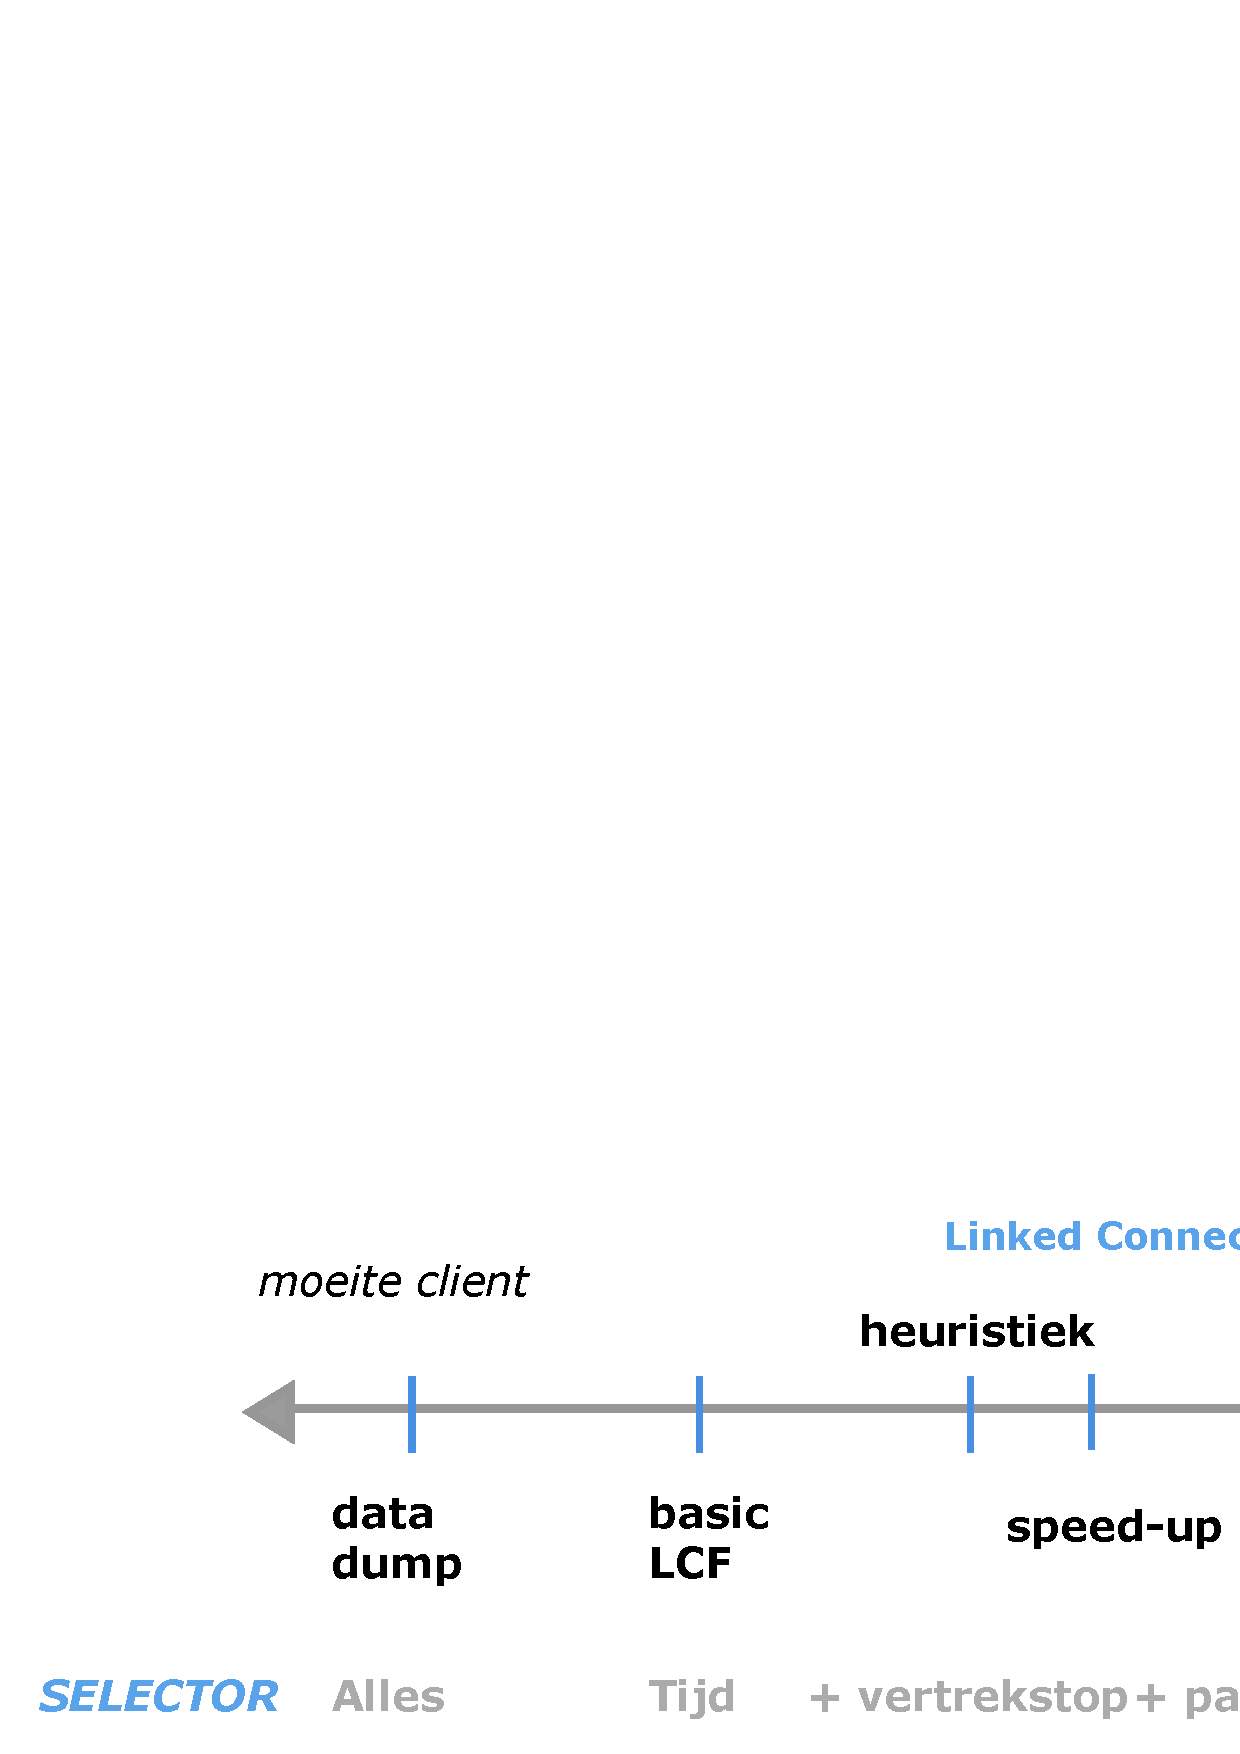
\includegraphics[scale=0.4]{LDF-asFinal.png}
\caption{Linked Data Fragmenten-as met optimalisatietechnieken}
\label{ldf-opt}
\end{figure}

Er werden twee nieuwe termen voor fragmenten ge\"introduceerd: basic Linked Connections Fragments en Neighbouring Linked Connections Fragments (NLCF). Dit laatste fragment maakt gebruik van de tijdsafstand tussen twee stops om connecties te filteren. Zowel de speed-up techniek als de heuristische techniek maken gebruik van deze NLCF's. Uit de resultaten \ref{table:gemiddeldesnelheid} en \ref{tijdmetcachingvolgensaantalstops} kan afgeleid worden dat dit het routeplannen hoogstens dubbel zo snel maakt.

De heuristische methode maakt enkel gebruik van NLCF. De cli\"ent is verantwoordelijk voor het kiezen van een volgende vertrekstop als het resultaat nog niet gevonden is. Om een goede afschatting te maken werd de belangrijkheid van een station gequoteerd aan de hand van het aantal rechtstreeks bereikbare stops. Dit kan makkelijk berekend worden tijdens het genereren van connecties. Bij deze techniek kan echter niet gegarandeerd worden dat de optimale oplossing gevonden wordt. Slechts 78\% van de queries werden optimaal opgelost. Dit kan als een future-work beschouwd worden (zie \ref{max-interval}).

De speed-up techniek garandeert wel dat de optimale oplossing gevonden wordt. De informatie van de eerste NLCF zorgt ervoor dat er minder connecties gescand moeten worden. Deze techniek maakt gebruik van paginering met hypermedia. Deze fragmenten zijn iets kostelijker om te berekenen voor de server. Dit is echter niet erg, omdat de server dynamisch de grootte van de pagina's en fragmenten kan aanpassen afhankelijk van de serverbelasting. Door een grotere fragmentgrootte te kiezen is het mogelijk om de querytijd te verdubbelen ten opzichte van de basis methode (figuren \ref{tijdmetcachingvolgensafstand} en \ref{tijdzondercachingvolgensaantalstops}).

Neighbouring Linked Connections Fragments vergt extra voorbewerking. Het berekenen van de minimale tijdsafstand tussen elke stop vergt weinig extra tijd, omdat dit gebeurt tijdens het genereren van connecties. De extra fase die het minimaal aantal overstappen $K$ berekend is optioneel als extra filter bij de heuristische methode. De heuristische methode geeft van elke stop binnen $K$ een reeks connecties binnen tijdsinterval $T$ terug. Bij grotere netwerken dan de NMBS kan het dus nodig zijn om toch een beperking hierop te stellen. De speed-up techniek beschouwt het aantal overstappen als maximaal om de snelste aankomsttijd te garanderen. Stations die minstens X aantal overstappen nodig hebben, bevinden zich hoogstwaarschijnlijk verder in de tijd waardoor deze connecties toch niet worden teruggeven in het eerste NLCF fragment.

Een andere optimalisatie is het dataverbruik. Door de extra tijdsafstandfilter worden minder nutteloze connecties teruggeven. Dit resulteert in 32\% minder dataverbruik bij de speed-up techniek en 27\% minder bij de heuristische methode. (zie \ref{table:dataverbruik}). In een \textit{real-world} omgeving zal dit waarschijnlijk nog een grotere rol spelen voor de snelheid.

Een laatste aspect die werd gerealiseerd is een \textit{merger} van verschillende connectiestromen. Die zorgt ervoor dat connecties van verschillende Linked Connections servers kunnen opgehaald worden door de cli\"ent. Om intermodaal te kunnen routeplannen moet er een systeem komen die informatie van  stopplaatsen van verschillende feeds semantisch kunnen beschrijven.

We kunnen concluderen dat we geslaagd zijn in op de opzet om client-side routeplannen sneller te maken zonder de garantie te verliezen dat de snelste route gevonden is. Niet alleen snelheid, maar ook dataverbruik is een stuk effici\"enter. Dit gaat ook niet ten koste van extra voorbewerkingstijd.

\chapter{Future work}

\section{Preprocessing}
\label{max-interval}
Tijdens de voorbewerkingsfase wordt voor elke stop de minimale afstand en overstappen tot elke buur bepaald. Een LC server moet connecties binnen een bepaald tijdsinterval teruggeven waarin de snelste route zich bevindt naar elke andere stop. Momenteel werd er verondersteld dat binnen een bepaald tijdsinterval $T$ elke snelste route bepaald kan worden. Een extra feature zou een afschatting zijn van het maximale tijdsinterval waarin connecties moeten teruggegeven worden voor elke stop. Kleine stops hebben bijvoorbeeld een regelmatige verbinding naar een groter station waaruit alle andere stations bereikbaar zijn. Als er binnen het halfuur een connectie bestaat, is het enkel nuttig om connecties binnen het halfuur op te vragen. Voor verafgelegen stations, zoals Basel voor de NBMS, is een groter tijdsinterval nodig.
Door deze informatie kan er met meer zekerheid en effici\"enter enkel de nuttige connecties teruggeven worden.

\section{Multicriteria queries}

Momenteel werd er enkel onderzocht hoe de snelste route gevonden kan worden. Een nieuwe pareto-optimale route zou kunnen beschouwd worden die ook rekening houdt met het maximaal aantal overstappen. CSA zou moeten aangepast worden zodat elke stop meerdere mogelijke oplossingen bijhoudt zodat er niet louter naar de tijd gekeken wordt, maar ook naar de trip. Voor de optimalisatie is dit ook een interessante uitbreiding wegens de manier de data werd voorbewerkt. Elke stop houdt de minimale tijd en het minimaal aantal overstappen naar elke andere stop bij. Er kan zo een extra HTTP parameter toegevoegd worden zodat de cli\"ent kan aanduiden hoeveel overstappen maximaal gemaakt mag worden.

Momenteel wordt er eerst een HTTP request gestuurd om de juiste URL te bekomen van een fragment. Er zou metadata in deze request toegevoegd kunnen worden over de stops die met 0, 1... overstappen bereikbaar zijn. Zo kan de cli\"ent een betere afschatting kunnen doen van het maximaal aantal overstappen.

\section{Intermodaliteit}

Een Linked Connections server is verantwoordelijk voor het aanbieden van connecties van een (of meerdere) provider(s). De cli\"ent moet zelf kunnen beslissen van welke providers data nuttig kan zijn. Een belangrijk aspect hierbij is metadata over stops. Momenteel zijn er geen afspraken over het gebruiken van vaste identifiers voor stops. Enkel zo kan er interoperabiliteit onstaan tussen datasets. Een cli\"ent moet weten of de identifier van de NMBS voor Antwerpen-Centraal dezelfde is als die van de Nederlandse Spoorwegen. Ook moet er geweten zijn welke operatoren en welke soort vervoersmiddelen actief zijn in bepaalde stations of met \textit{footpaths} bereikbaar zijn. 

Een volgende stap zou het combineren zijn van bussen (De Lijn) en treinen (NMBS) die actief zijn binnen dezelfde regio. Er moet gemodelleerd worden wanneer het nuttig is om bepaalde modaliteiten te gebruiken. Het is bijvoorbeeld logisch om bij grote afstanden eerst de trein te nemen en daarna de bus. Desnoods met een bus naar het vertrekstation. Hieruit blijkt dat de vraag naar metadata steeds groter zal zijn. Enkele voorbeelden:

\begin{itemize}
\item faciliteiten zoals rolstoeltoegankelijkheid
\item locatie van perrons
\item mogelijke wandelafstanden
\item gebied waar de publieke vervoersmaatschappij actief is, bijvoorbeeld in GeoJSON-formaat
\item welk soort voertuig
\end{itemize}

Op basis van deze metadata kan een cli\"ent slimme beslissingen nemen om connecties op te halen van de juiste providers. Met behulp van de \textit{merger} die in hoofdstuk \ref{merger} besproken wordt, kunnen de connecties makkelijk gesorteerd samengevoegd worden voor CSA.

\section{Grote netwerken}

Het Connection Scan Algorithm (CSA) is niet schaalbaar voor zeer grote netwerken. Linked Connections werkt snel voor lokale netwerken. Een oplossing hiervoor is  accelerated CSA die we besproken hebben in de literatuurstudie (\ref{acsa}). Deze optimalisatie vereist echter preprocessing. Dit zou toepasbaar kunnen worden binnen Linked Connections door een \textit{accelareted} Linked Connections server te ontwerpen. Wanneer de cli\"ent wil query'en over lange afstanden kan dit eerst hierop gedaan worden. Voor lokale queries kan er dan op de huidige implementatie overgeschakeld worden. 

\subsection{Realtime informatie}

Extra transformer toevoegen die trip van connectie checkt -> update -> hersorteren wel


% appendices
\appendix

% hier worden de appendices ingevoegd (\includes)


% \include{referenties}

\bibliographystyle{plain}
\bibliography{lc-referenties}

\backmatter

% eventueel: lijst van figuren en tabellen
\listoffigures
\listoftables

% lege pagina (!!)

% kaft

\end{document}
